\documentclass[uplatex,dvipdfmx]{bxjsarticle}

\usepackage{listings}
\usepackage{xcolor}
\usepackage[hidelinks]{hyperref}
\usepackage{graphicx}
\usepackage{amsmath}
\usepackage{geometry}
\geometry{margin=25mm}

\usepackage{tcolorbox}
\newtcbox{\code}[1][]{
  colback=gray!10!white,
  colframe=gray!20!white,
  boxrule=1pt,
  left=0mm,right=0mm,top=0mm,bottom=0mm,
  box align=base,
  nobeforeafter,
  fontupper=\ttfamily
}


% Ciscoコマンド用の設定
\lstdefinelanguage{Cisco}{
  morekeywords={enable,configure,terminal,interface,router,network,ip,route,show,version,exit,no,auto-summary},
  sensitive=false,
  morecomment=[l]{!},
  morestring=[b]",
}

\lstset{
  language=Cisco,
  basicstyle=\ttfamily\small,
  keywordstyle=\color{blue}\bfseries,
  commentstyle=\color{gray},
  stringstyle=\color{orange},
  backgroundcolor=\color{gray!10},
  frame=single,
  breaklines=true,
  captionpos=b,
  numbers=left,
  numberstyle=\tiny\color{gray},
  xleftmargin=1.5em,
  xrightmargin=1.5em
}

\title{Ciscoルーター設定備忘録}
\author{Yuiki Nakanishi\\Ito Nagahama}
\date{\today}

\begin{document}

\maketitle

\section{$\sim$ 前期中間}

\subsection{ケーブルの種類}

同じ種類のケーブルを接続する場合はクロスケーブル,違う種類の場合はストレートケーブル.

\begin{figure}[htbp]
  \centering
  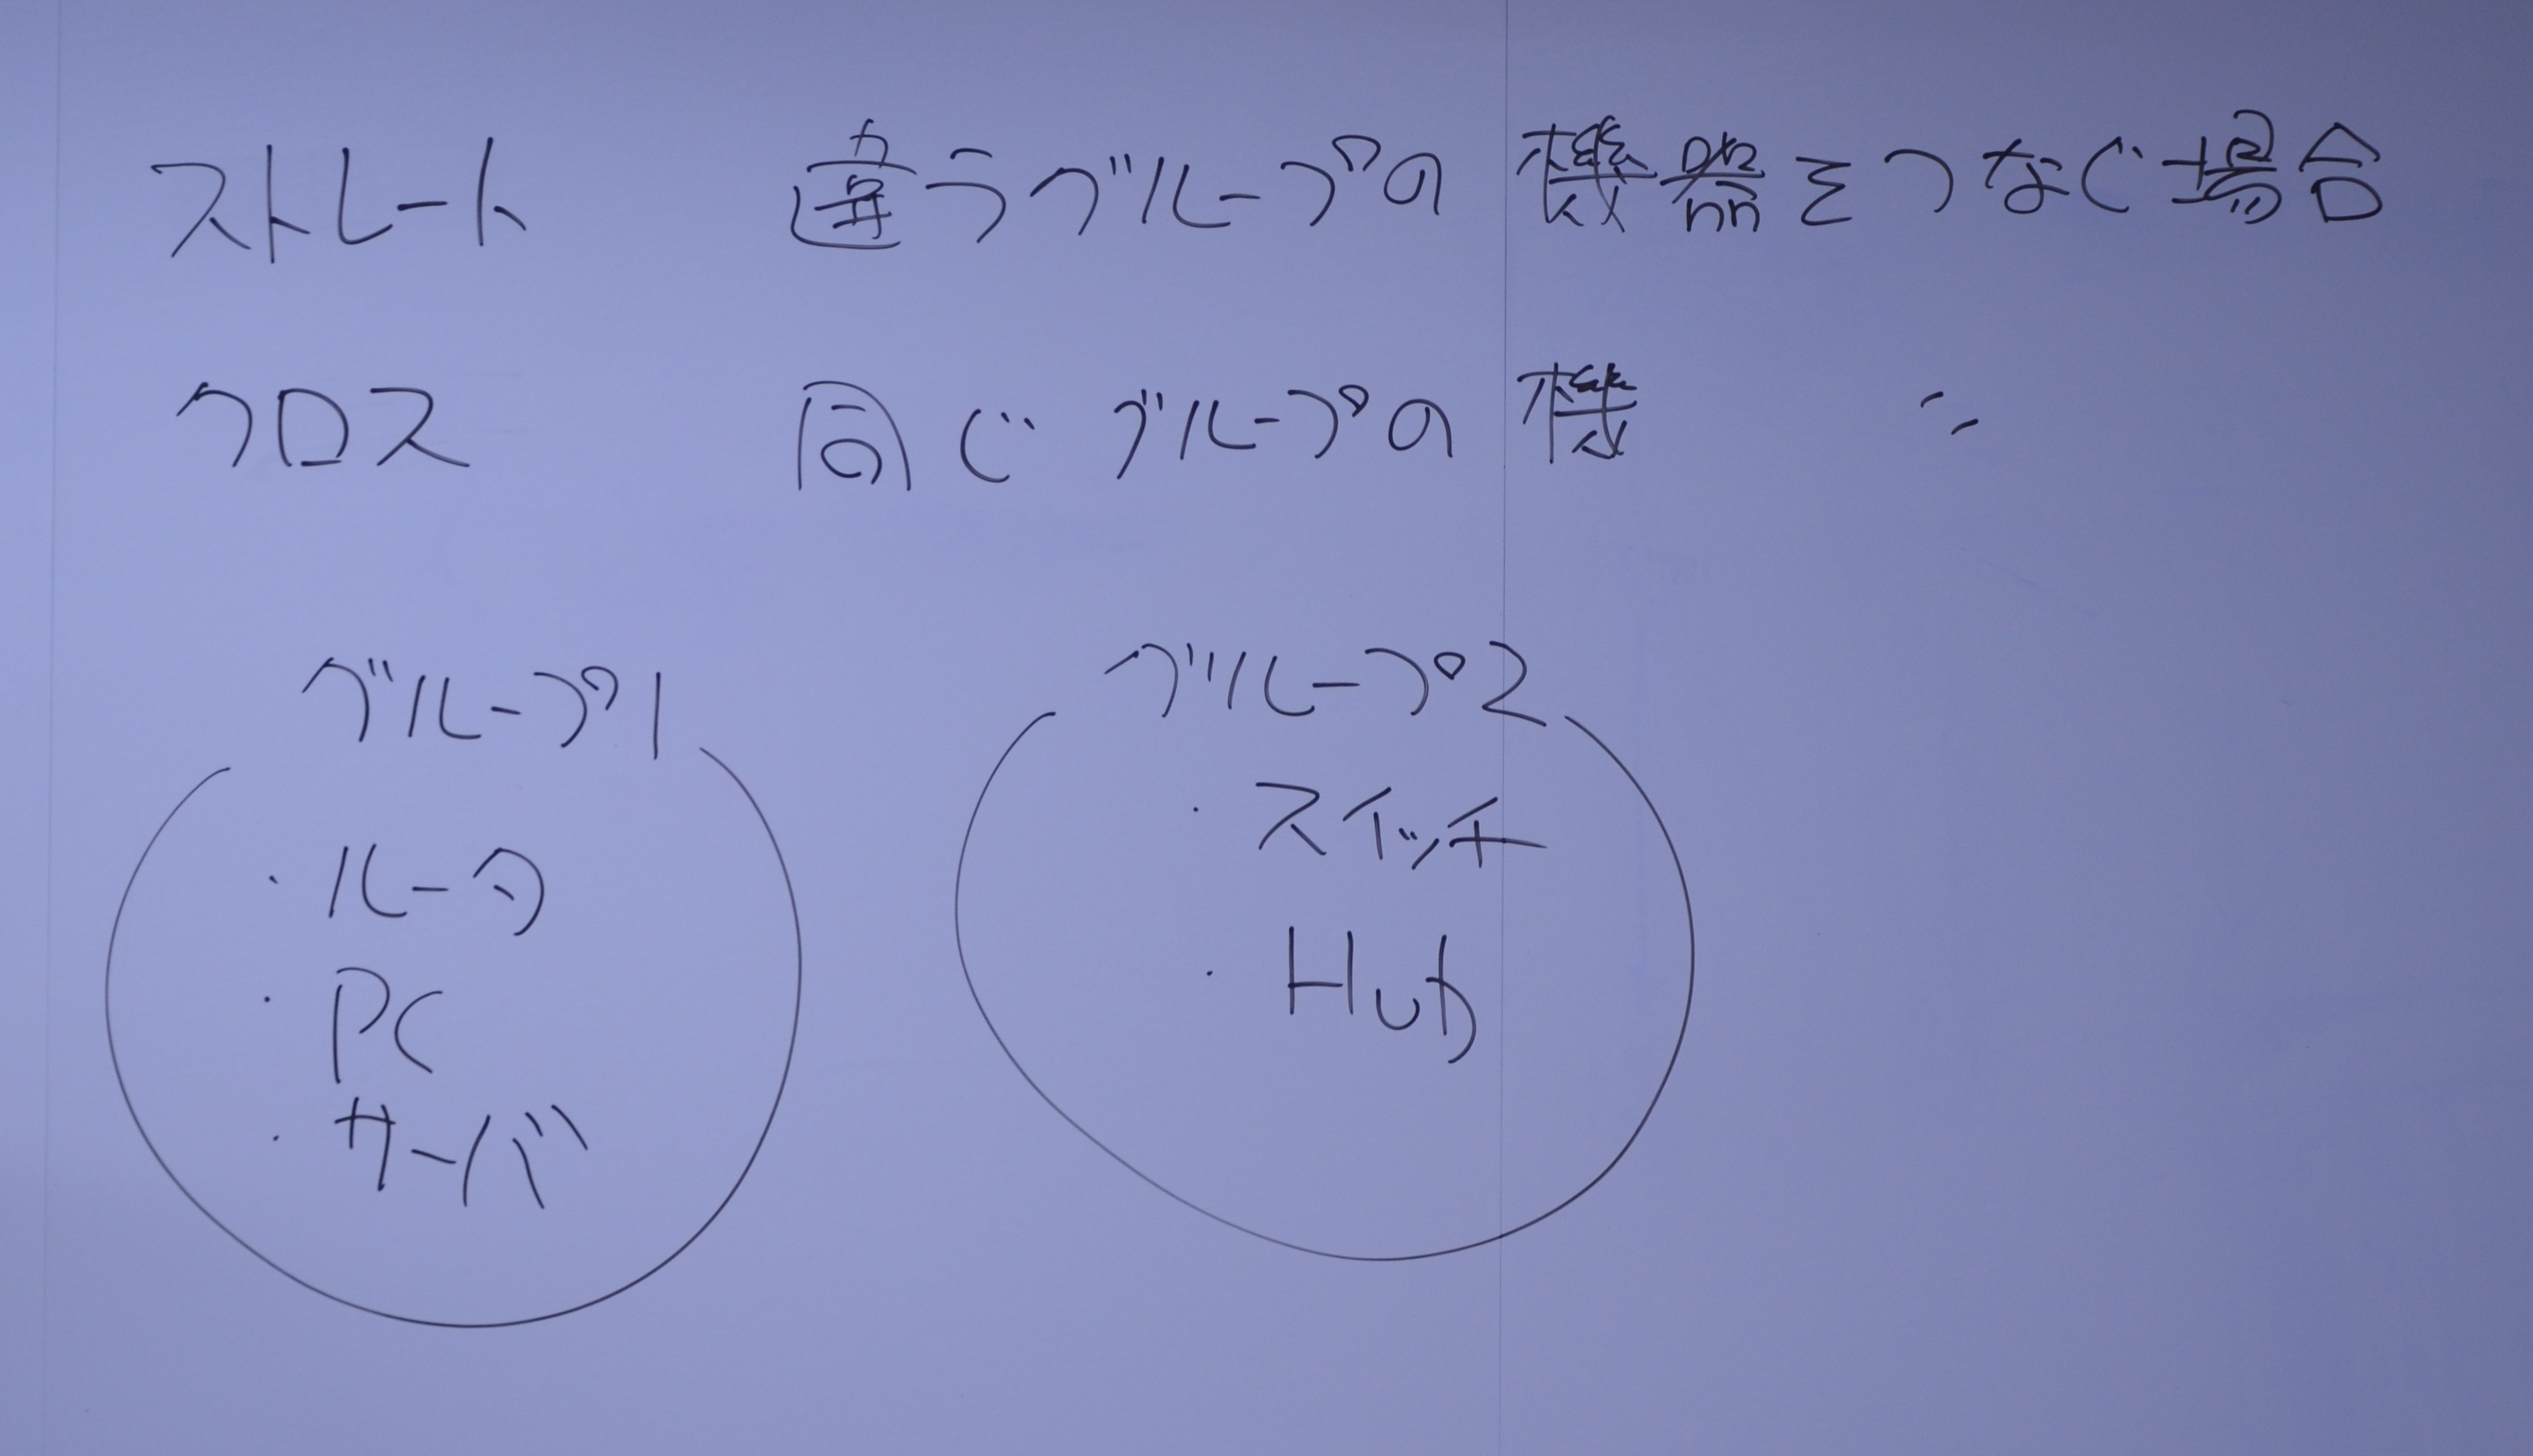
\includegraphics[width=1\linewidth]{figure/lan.JPG}
\end{figure}

\subsection{モードの移動}

\subsubsection{管理者になる}

\begin{lstlisting}[caption={管理者になる}]
> enable
\end{lstlisting}

\subsubsection{コンフィグモードに入る}

\begin{lstlisting}[caption={コンフィグモードに入る}]
# config terminal
\end{lstlisting}

\subsection{ホスト名の変更}

\begin{lstlisting}[caption={ホスト名の変更}]
(config) hostname XX  // hostname を XX に変更する.
\end{lstlisting}

\subsection{IP Address 設定}

\begin{lstlisting}[caption=IP Address Settings]
en
conf t
int fa ?/?  // LAN ポート番号
ip address 192.168.1.0  255.255.255.0 // IP Address,Subnet Mask
no shut
\end{lstlisting}

\subsection{設定の管理}

\subsubsection{設定の表示}

\begin{lstlisting}[caption={設定の表示}]
# show running-config
\end{lstlisting}

\subsubsection{保存されている設定の表示}

\begin{lstlisting}[caption={保存されている設定の表示}]
# show startup-config
\end{lstlisting}

\subsubsection{設定の保存}

\begin{lstlisting}[caption={設定の保存}]
# copy running-config startup-config
\end{lstlisting}

\subsection{パスワードの設定}

\subsubsection{管理者のパスワード}

\begin{lstlisting}[caption={管理者のパスワード}]
(config#) enable secret XXXX  // XXXX というパスワードを設定する.
\end{lstlisting}

\subsubsection{コンソールのパスワード}

\begin{lstlisting}[caption={コンソールのパスワード}]
(config)# line con 0
(config-line)# password XXXX
(config-line)# login
\end{lstlisting}

\subsubsection{TELNET のパスワード}

\begin{lstlisting}[caption={TELNET のパスワード}]
(config)# line vty 0 4
(config-line)# password XXXX
(config-line)# login
(config)# service password-encryption
\end{lstlisting}

\subsection{スタティックルートの設定}

\begin{lstlisting}[caption={スタティックルートの設定}]
(config)# ip route 宛先ネットワークアドレス 宛先サブネットマスク ネクストホップ
// 設定を削除する場合
(config)# no ip route xxx.xxx.xxx.xxx yyy.yyy.yyy.yyy zzz.zzz.zzz.zzz
\end{lstlisting}

\subsection{デフォルトルートの設定}

\begin{lstlisting}[caption={デフォルトルートの設定}]
(config)# ip route 0.0.0.0 0.0.0.0 <ネクストホップ>

\end{lstlisting}

\subsection{RIPの設定}

RIPの設定は以下の通りです。

\begin{lstlisting}[caption=RIP Settings,label=rip_def]
router rip
network 192.168.1.0 // ルータにつながっている全ての IP Address を記述する.
\end{lstlisting}

設定中のコマンドは、例えば \texttt{router rip} や \texttt{no auto-summary} のように行中に記述できます。

\subsection{EIGRPの設定}

\begin{lstlisting}[caption=EIGRP Settings,label=eigrp_def]
router eigrp 100
network 192.168.1.0 // ルータにつながっている全ての IP Address を記述する.
\end{lstlisting}

\subsection{Changing Administrative Distance}

ルーティングプロトコルの優先順位

\begin{lstlisting}[caption=Changing Administrative Distance]
router rip
distance 80 // 1 が最も優先順位が高い
\end{lstlisting}

\section{$\sim$ 前期末}

\subsection{RIP $\cdot$ EIGRP}

ネットワークが分割されている場合の通信

例えば,\code{192.168.1.0/24} のネットワークを二分割して,\code{192.168.1.0/25} と \code{192.168.1.128/25} に分割する場合などである.

その場合,それぞれ Listing \ref{rip_def}, \ref{eigrp_def} のように通常設定後以下の設定をする.

\begin{lstlisting}
(config) # router rip
(config-router) # version 2
(config-router) # no auto-summary
\end{lstlisting}

\code{version 2} にすることによって分割したネットワークが使えるようになる.
\code{no auto-summary}によって \code{auto-summary} 機能を使えなくする.
この時に直接接続されていないルータでも \code{no auto-summary} にすること!

\textbf{注意}\\
\begin{itemize}
  \item \code{version 2 から元に戻すとき}
  \begin{description}
    \item[〇] \code{no version 2}
    \item[×] \code{version 1} 
  \end{description}
  \item \code{auto-summary} に戻すとき
  \begin{description}
    \item[〇] \code{auto-summary}
  \end{description}
\end{itemize}

\code{auto-summary} のほうがルーティングテーブルが小さくなるためなるべく \code{auto-summary} を使用する.\\

\begin{tcolorbox}[title=Point,colback=yellow!10,colframe=black,boxrule=0.8pt,arc=2mm]
一つのネットワークを分割してかつ離れた場所に置いた場合に \code{no auto-summary} \\
それ以外は \code{auto-summary} のまま
\end{tcolorbox}




\section{$\sim$ 後期中間}
\section{$\sim$ 学年末}

\end{document}
